\subsection{Purpose} 
The following \textit{Requirements Analysis and Specification Document} examines a possible solution for a specific system-to-be provided by the TrackMe company. Therefore, this document contains the description of the scenarios, the use cases that describe them, and the models describing requirements and specification for the system-to-be.
\bigbreak
\noindent
Data4Help is a location-based health information service-to-be that allows third parties to monitor the location and health status of individuals. The given problem is to design and develop this service and other two services, AutomatedSOS and Track4Run, which exploit the features offered by the first one.
\bigbreak
\noindent
AutomatedSOS is a service-to-be thought to help elderly people. Constantly monitoring the health status of the subscribed customers, this service sends to the user's location an ambulance as soon as the recorded values are anomalous, for example when some health parameters are below certain thresholds.
\bigbreak
\noindent
Finally, Track4Run is a service-to-be that tracks athletes participating in a run. The service, allows organizers to define the path for the run, participants to enroll to the run and spectators to see on a map the position of all the runners during the run.
\subsection{Scope}
\subsubsection{Goals}

\begin{enumerate}
\item[•] {\Large Data4Help}
	\begin{enumerate}
		\item [G.1] Acquire user's position and health status.
		\item [G.2] Provide to third parties user's position and health status.
		\begin{enumerate}
		\item [G.2.1] Provide data on demand to non-subscribed third parties.
		\item [G.2.2] Provide data in real-time to subscribed third parties.
		\end{enumerate}
		\item [G.3] Allow third parties two different ways to get user's data.
		\begin{enumerate}
		\item [G.3.1] Allow third parties to get data of a single person.
		\item [G.3.2] Allow third parties to get data of a group of people.
		\end{enumerate}
		\item [G.4] Provide data in an anonymous way, to protect user's privacy.
	\end{enumerate}
	
\item[•] {\Large AutomatedSOS}
	\begin{enumerate}
		\item [G.5] Retrieve user's position and health status.
		\item [G.6] Monitor user's health parameters.
		\item [G.7] Send an ambulance to user's location whenever certain parameters are below the threshold.
		\end{enumerate}
	
\item[•] {\Large Track4Run}	
	\begin{enumerate}
		\item [G.5] Retrieve user's position and health status.
		\item [G.8] Allow promoters to manage a run.
		\begin{enumerate}
		\item [G.8.1] Allow promoters to define the path for the run. 
		\item [G.8.2] Allow promoters to invite athletes to the run. 
		\end{enumerate}
		\item [G.9] Allow athletes to enroll on a specific run.
		\item [G.10] Allow spectators to watch in real time the position of every athlete in a specific run.
	\end{enumerate}
\end{enumerate}

\subsubsection{World Phenomena}
\begin{figure}[H]
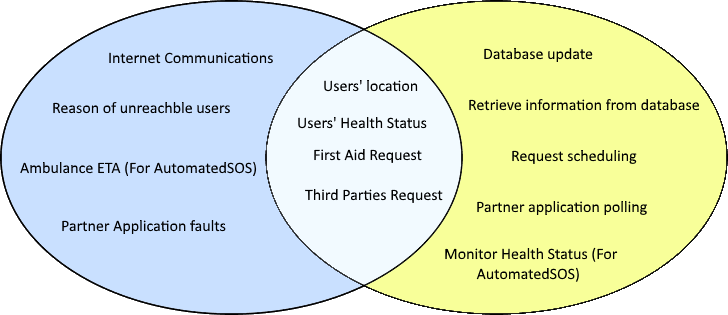
\includegraphics[scale=0.8]{Images/WordPhen.png}
\caption{World Phenomena}
\end{figure}

\subsection{Definitions, Acronyms, Abbreviations}

\begin{enumerate}
\item[•] {\Large Definitions}
	\begin{enumerate}
		\item Individual monitoring request: request to access to the data of some specific  individuals.
		\item Group monitoring request: request to access to anonymized data of groups of individuals.
		\item Live/real-time acquisition: third parties can access to data as soon they are ready, 				through service updates.
		\item On demand acquisition: third parties can access to data when they request 				them.
		\item User credentials: information that an individual has to provide to become a 				registered user: name, surname, date of birth, address, email, telephone.
			number, job, marital status and fiscal code. 
		\item Third parties' credentials: information that a company has to provide to 					become a registered one: company name, p.iva.
		\item Run information: all the information about the run such as name, date, promoters, 				maximum number of participants and race path.
		\item Partner Application: Application installed on users' device, not necessarily developed by TrackMe, that is in charge with retrieve location and health status. 
		\item Security Number / Fiscal Code: a Social Security Number (SSN) is a nine-digit number issued to U.S. citizens and its primary purpose is to track individuals. Fiscal Code is the equivalent of Social Security Number in Italy.
	\end{enumerate}
\end{enumerate}

\newpage
\subsection{Revision History}
This is a report on all versions of the document along with the reason of the updates/changes.

\begin{table}[h]
\begin{tabular}{|l|p{.45\textwidth}|p{.45\textwidth}|}
\hline
Version & Changes & Motivation\\ \hline
1.1     & Corrected orthographic errors. & / \\ \hline
 & Added text assumptions, modified use cases, mock-ups, requirements and class diagram. & In the first version of the document Data4Help would also answer to third party requests with data retrieved by AutomatedSOS, leading to major exploitation of very sensitive data.   \\ \hline
 & Modified Product Functions, requirements, text assumptions and use cases. & In the first version of the document Data4Help provided only raw data as answers to third parties' requests. Statistics could also be useful.  \\ \hline
 & Modified requirements, mock-ups, product functions, text assumptions and use cases. & In the first version of the document the logic behind promoting and enrolling to a run event wasn't explained enough. \\ \hline
\end{tabular}
\caption{Version 1.1}
\end{table}

\begin{table}[h]
\begin{tabular}{|l|p{.45\textwidth}|p{.45\textwidth}|}
\hline
Version & Changes & Motivation\\ \hline
1.2     & Corrected orthographic errors. & /  \\ \hline
& Modified use-cases and use-case diagrams & In the new version of the document is fixed an incongruence about the subscription to a group.  \\ \hline
 & Modified requirements & In the new version of the document is better specified the role of each requirements deleting all the repeated ones.   \\ \hline
 & Modified mock-ups & In this version of the document is added a new web page in user interface sector for third parties. \\ \hline
  & Modified definitions & \ \\ \hline
\end{tabular}
\caption{Version 1.2}
\end{table}

\clearpage
\subsection{Document Structure}
This document is composed by six sections:

\begin{center}
\centering
\begin{table}[H]
\centering
\begin{tabular} { p{4cm}  p{10 cm} }
\toprule
\textbf{1. Introduction} & This section gives an introduction to the problem and describes the purposes of the services-to-be provided by TrackMe. The scope of the application is defined by describing the application domain and listing the goals. \\ \midrule
\textbf{2. Overall Description} & This section presents the overall description of the project. \textit{Product perspective} subsection presents the class diagram describing the domain model used by all the three services. In addition, that subsection includes a state diagram that analyzes the process of making a request to access the users' data. \textit{User characteristics} subsection lists the actors interested in using these services. \\ \midrule
\textbf{3. Specific Requirements} &  This section specifics the requirements identified, both functional and non functional. The first subsection includes the external interface requirements, showing user interfaces with several mockups. Some scenarios describing specific situations are then listed here. The functional requirements are defined by using use case and sequence diagram. The non functional requirements are defined through performance requirements, design constraints and software system attributes.  \\ \midrule
\textbf{4. Formal Analysis Using Alloy}  & This section includes the alloy model and the discussion of its purpose. Also, a world generated by it is shown. \\ \midrule
\textbf {5. Effort Spent} & This section include information about the number of hours each group member has worked for this document. \\ \midrule
\textbf{6. Reference Documents} & This section contains the list of reference documents. \\ \bottomrule
\end{tabular}
\caption{Document Structure}
\end{table}
\clearpage
\end{center}
\clearpage